% -------------------------------------------------------------------------------- %

\begin{exercise}

With an n-step method, the value estimates do change from step to step, so an algorithm that used the sum of TD errors (see previous exercise) in place of the error in (7.2) would actually be slightly different algorithm. Would it be a better algorithm or a worse one? Devise and program a small experiment to answer this question empirically.

\end{exercise}

% -------------------------------------------------------------------------------- %

\begin{solution}

We do our experiment with an environment consisting of three States $S_1,S_2$ and $S_3$ where we always start in $S_1$ and $S_3$ is our terminal state. From state $S_1$ we have two actions, one leads us back into $S_1$ with probability $0.9$ and leads to $S_2$ with probability $0.1$. From state $S_2$ we transition back into $S_1$ with a probability of $0.9$ or end the episode with a transition into $S_3$ with probability $0.1$. We get a reward of $0$ for all transitions but the transition into the terminal state, where we get a reward of $1$.

We can easily calculate the real state-value function under this policy and the following graphs show the results of the algorithm as given in the book vs the algorithm where we use the sum of TD errors for different values of $\alpha$ and $\gamma$.
\begin{center}
  \begin{figure}[H]
    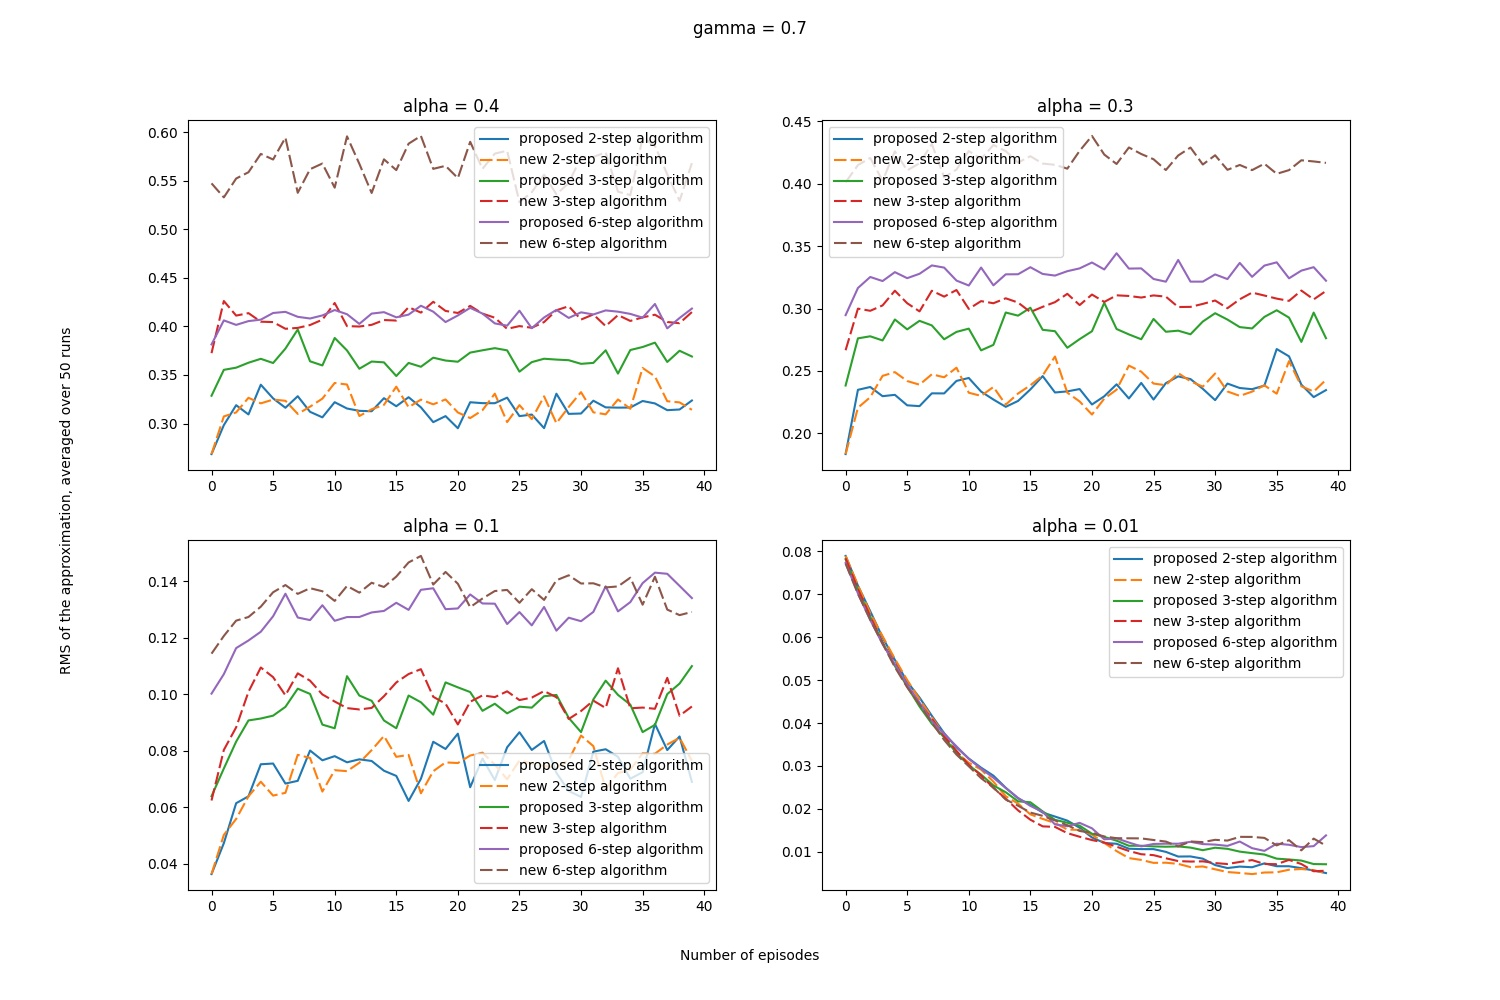
\includegraphics[width = 0.9 \textwidth]{gamma=0,7.jpg}
    \caption{The error for different values of $\alpha$ with $\gamma = 0,7$}
  \end{figure}

  \begin{figure}[H]
  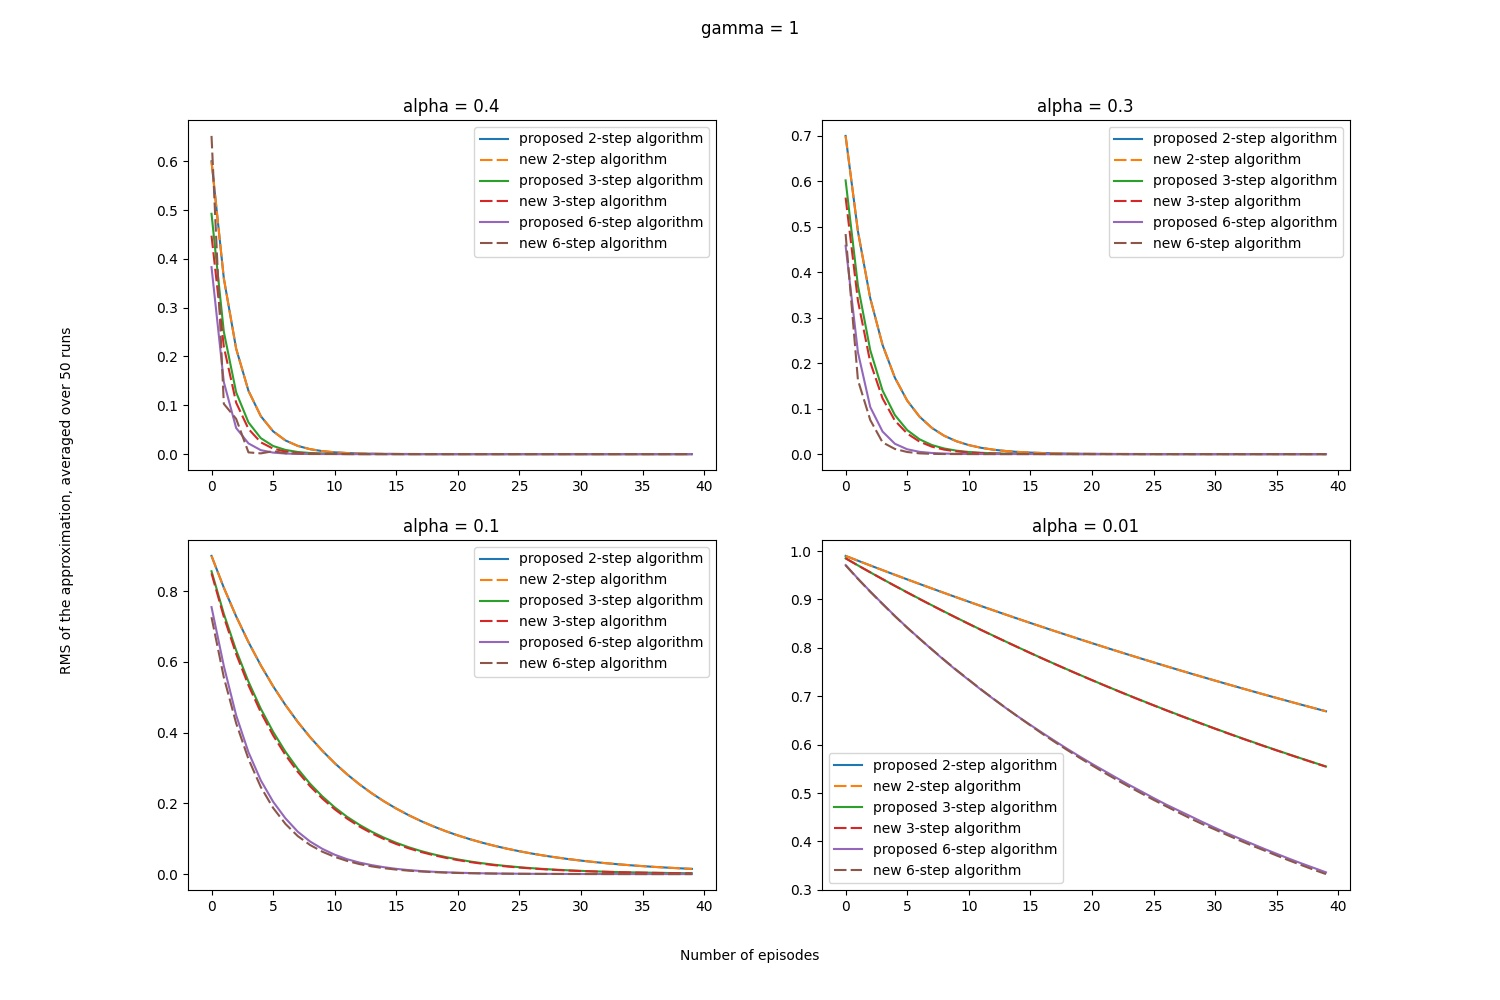
\includegraphics[width = 0.9 \textwidth]{gamma=1.jpg}
    \caption{The error for different values of $\alpha$ with $\gamma = 1$}
  \end{figure}
\end{center}

For the values of $\alpha$ and $\gamma$ where the approximations converge to the real values, the new algorithm seems to do slightly better, while it does worse in the other case. What is also interesting to see, is that the lower $n$-step methods give a better approximation in those cases, where the algorithm does not seem to fully converge.
\end{solution}

% -------------------------------------------------------------------------------- %
